\documentclass[11pt]{article}
\usepackage{tocloft}
\usepackage{graphicx}
\usepackage{calc}
\usepackage{amssymb}
\usepackage{color}
\usepackage{array}
\usepackage[sc]{mathpazo}
\usepackage{url}
\usepackage[final]{pdfpages}
\usepackage{amsmath}

%\linespread{1.05}
\oddsidemargin=0pt
\evensidemargin=0pt
\textwidth=6.5in
\topmargin=0pt
\headheight=0pt
\headsep=0pt
\textheight=9in
% EXPERIMENTAL
%\parindent=0pt
%\parskip=3pt
\setlength{\parindent}{0cm}
\newcommand\secfont{\fontfamily{cmss}\selectfont}%\textwidth 5.5truein
\newcommand\pifheading[1]{{\secfont\textbf{#1}:}}
%\oddsidemargin -0.40truein
%\textheight 8.0truein
%\topmargin -0.25truein
\def\lo{
\mathrel{\raise.3ex\hbox{$<$}\mkern-14mu\lower0.6ex\hbox{$\sim$}}
}
\def\hi{
\mathrel{\raise.3ex\hbox{$>$}\mkern-14mu\lower0.6ex\hbox{$\sim$}}
}

\textwidth = 6.6 in
\textheight = 9.1 in
\oddsidemargin = -0.05 in
\evensidemargin = +0.05 in
\topmargin = -.1 in
\headheight = 0.0 in
\headsep = 0.0 in
\parskip = 0.06in
\newcommand\registered{{\ooalign{\hfil\raise .00ex\hbox{\scriptsize R}\hfil\crcr\mathhexbox20D}}}

%% Define a new 'leo' style for the package that will use a smaller font.
\makeatletter
\def\url@leostyle{%
  \@ifundefined{selectfont}{\def\UrlFont{\sf}}{\def\UrlFont{\small\ttfamily}}}
\makeatother
%% Now actually use the newly defined style.
\urlstyle{leostyle}

%\pagestyle{empty}
%\includeonly{previous,proposal_references}
%\includeonly{proposal_references}
%\includeonly{previous}

% TOC

\begin{document}
%%%%%%%%%%%%%%%%%%%%%%%%%%%%%%%%%%%%%%%%%%%%%%%%%%%%%%%%%%%%%%%%%%%%%
\begin{center}
\textbf{\Large
AST101: Our Place in the Universe \\
\vspace*{0.1cm}
Lab 10: Planets' Temperature Prelab 
}
\end{center}

\vspace*{0.5cm}

{\Large Name:}\vspace*{0.5cm}\\\hrule
{\Large Student number (SUID):}\vspace*{0.5cm}\\\hrule
{\Large Lab section:}\vspace*{0.5cm}\\\hrule
\vspace*{0.5cm}

%%%%%%%%%%%%%%%%%%%%%%%%%%%%%%%%%%%%%%%%%%%%%%%%%%%%%%%%%%%%%%%%%%%%%
\section{Introduction}

In this lab, we'll be exploring why the planets have the temperatures that they do. You'll be doing a calculation in your 
lab to figure out the temperatures of several of the Solar System planets; as preparation, think about and answer the 
following.

\section{Energy balance}

Suppose you have a beaker of water with an electric heating element in the bottom. When this heating element is turned on, it delivers
1000 watts of power to the water. However, if the water is warmer than the room, it will be constantly
{\it losing} heat as well -- the warmer the water, the faster it loses heat.

{\bf Question 1:} Suppose that you turn the heater on, and at its current temperature the water loses heat at a rate of 
800 watts. What will happen to the temperature of the water as time passes?

\vspace{1in}

{\bf Question 2:} Suppose that the water is warmer than this, and at its warmer temperature the water loses heat at a rate
of 1200 watts. In this case, what will happen to the temperature of the water as time passes?

\vspace{1in}\newpage
{\bf Question 3:} Suppose that the rate of heat loss and the temperature are related as shown here. Now suppose that you
turn the heater on and let it sit for a long time. What will the equilibrium temperature of the water be?

\begin{center}
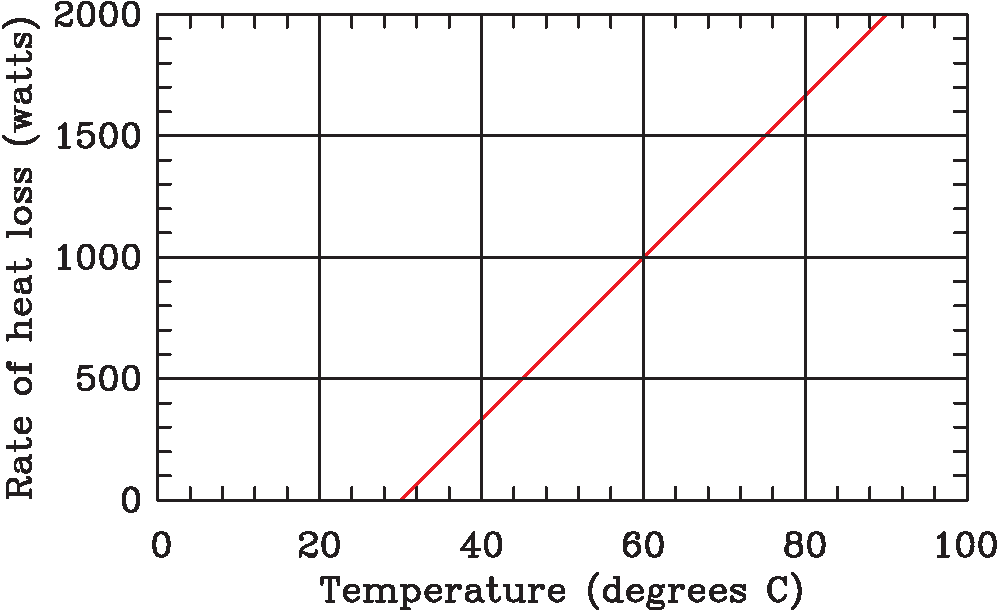
\includegraphics[width=3in]{heat-loss.pdf}
\end{center}

\vspace{1in}
{\bf Question 4:} Explain in words how you figured out Question 3. What must be true when an object is at its equilibrium
temperature?

\vspace{1in}
{\bf Question 5:} In the previous problems, the mechanism to add heat to the water was an electric heater, and the 
mechanism by which it lost heat was conduction through the walls of the beaker. Would your answer to Question 4 
be different if the processes that added and removed heat from the beaker were changed? (Suppose we heated it up by
putting it out in the sunlight, for instance.)

\vspace{1in}
\section{Things spreading out}

Suppose that I have a flashlight that emits a beam of light in the shape of a square. It emits a total of 
100 watts of light.

The rigorous way to talk about brightness is as an {\it intensity} -- the number of watts per square meter of light.
If you know the total amount of light, you can calculate intensity by dividing the total amount of light (in watts)
by the area (in square meters). This will tell you the intensity of the light (in watts per square meter).
\newpage
{\bf Question 6:} Suppose that if I hold the flashlight a distance $d$ away from a wall, it makes a square patch of light
that is one meter on a side. What is the {\it area} of the lit region of the wall?

\vspace{1in}
{\bf Question 7:} What is the {\it intensity} of the lit patch on the wall?

\vspace{1in}
{\bf Question 8:} Now suppose that I hold the flashlight twice as far away from the wall, at a distance $2d$. When I do that,
the light will spread out more, so that the lit patch is now a square two meters on a side. {\it Now} what is the area 
of the lit patch? What is its intensity?

\vspace{1in}
{\bf Question 9:} Now suppose that I get {\it ten} times further away -- at a distance $10d$ from the wall. What will the
intensity of the lit patch on the wall be now? 

\vspace{1in}
{\bf Question 10:} Fill in the blank in the following: {\it If I move $x$ times further away from the wall, the 
intensity of the light on the wall gets \underline{\hspace{1in}} times weaker}. 

\vspace{1in}
{\bf Question 11:} Based on the above, why do you think that Earth is hotter than Pluto?

\vspace{1in}
\section{An algebra reminder}

{\bf Question 12:} Can you simplify the expression $\frac{1}{4} x^4$ by cancelling the $1/4$ with the $4$? Why or why not?

\vspace{1in}

{\bf Question 13:} What is \


\end{document}

